\chapter {Graph Theory}
\label{chap:graphTheory}
\myTop{This chapter regards the graph theory in relation to the Rubik's Cube. There will be a description of the shortest path and calculation of the diameter of a graph. The chapter will end in an example using a much smaller Rubik's Cube graph; the Middle movement graph.}

A graph consists of a set of vertices, $V$ \cite[p. 592]{Rosen07}, and a set of edges, $E$. There are several types of graphs, but in this chapter only simple graphs are described. This means the graph is undirected, has no loops and their can only be one edge between two vertices. Since all weights are 1 the graphs can be considered non-weighted.

\section{Shortest Path}
The shortest path from one vertice to another in a graph can be found by checking the length of each possible path. This is easy for small graph such as the one described in subsection \ref{sub:middleMoveGroup} but for bigger graph such as the \rubik{} graph this is practically impossible. 

The shortest path between two vertices can be found with Dijkstra's Algorithm \cite[p. 651]{Rosen07}. The description of the algorithm is omitted for brevity. Dijkstra's Algorithm takes an weighted graph and two vertices as input. Because of this the \rubik{} graph has to be weighted. Since each move contributes to the total number of moves by the same number, one, each edge is given the weight 1. The weight will be omitted in every illustration in this chapter because they are all 1.  

\section{Solving the Diameter}
To find the diameter of a graph is to find the longest shortest path between any two vertices in the given graph. This can be done by using Dijkstra's Algorithm on every set of vertices in the graph. This can be applied to the \rubik{} graph as well and finding the maximum number of \twist{}s to solve the \rubik{} in the worst case scenario. %Unfortunately this approach is not viable because of the tremendous amount of positions the \rubik{} has even when considering symmetries.

%The diameter of the \rubik{} graph can be found be finding where the upper and lower bound meet with some other method.

\section{Describing the Cube as a Graph}
In order to describe the \rubik{} as a graph it is necessary to determine the edges and the vertices. In this example each edge of the graph represents a \twist{} and a vertices represent the positions.  The full \rubik{} graph is indeed a simple graph. A move can be reversed, hence no directions. In order to get from a position $a$ to a position $b$, adjacent to $a$, you can only get their by one move. Unless you take a detour trough one or several other positions. The full \rubik{} graph consist of $4.5\cdot10^{19}$ vertices and all having 18 edges. It is practically impossible to draw this graph. Therefore the graph will be explained with a much simpler graph; the Middle Movement Group.


\subsection{The Middle Movement Graph}
\label{sub:middleMoveGroup}
This graph is a \rubik{} graph consisting of only the moves that \twist{}s the middle sections. This is R2m F2m U2m. Note: R2m = R2 L2.  This graph is fairly small, since it only consist of eight vertices and 12 edges. See figure \ref{fig:graphMiddleSlice2}.

\begin{figure}
	\centering
		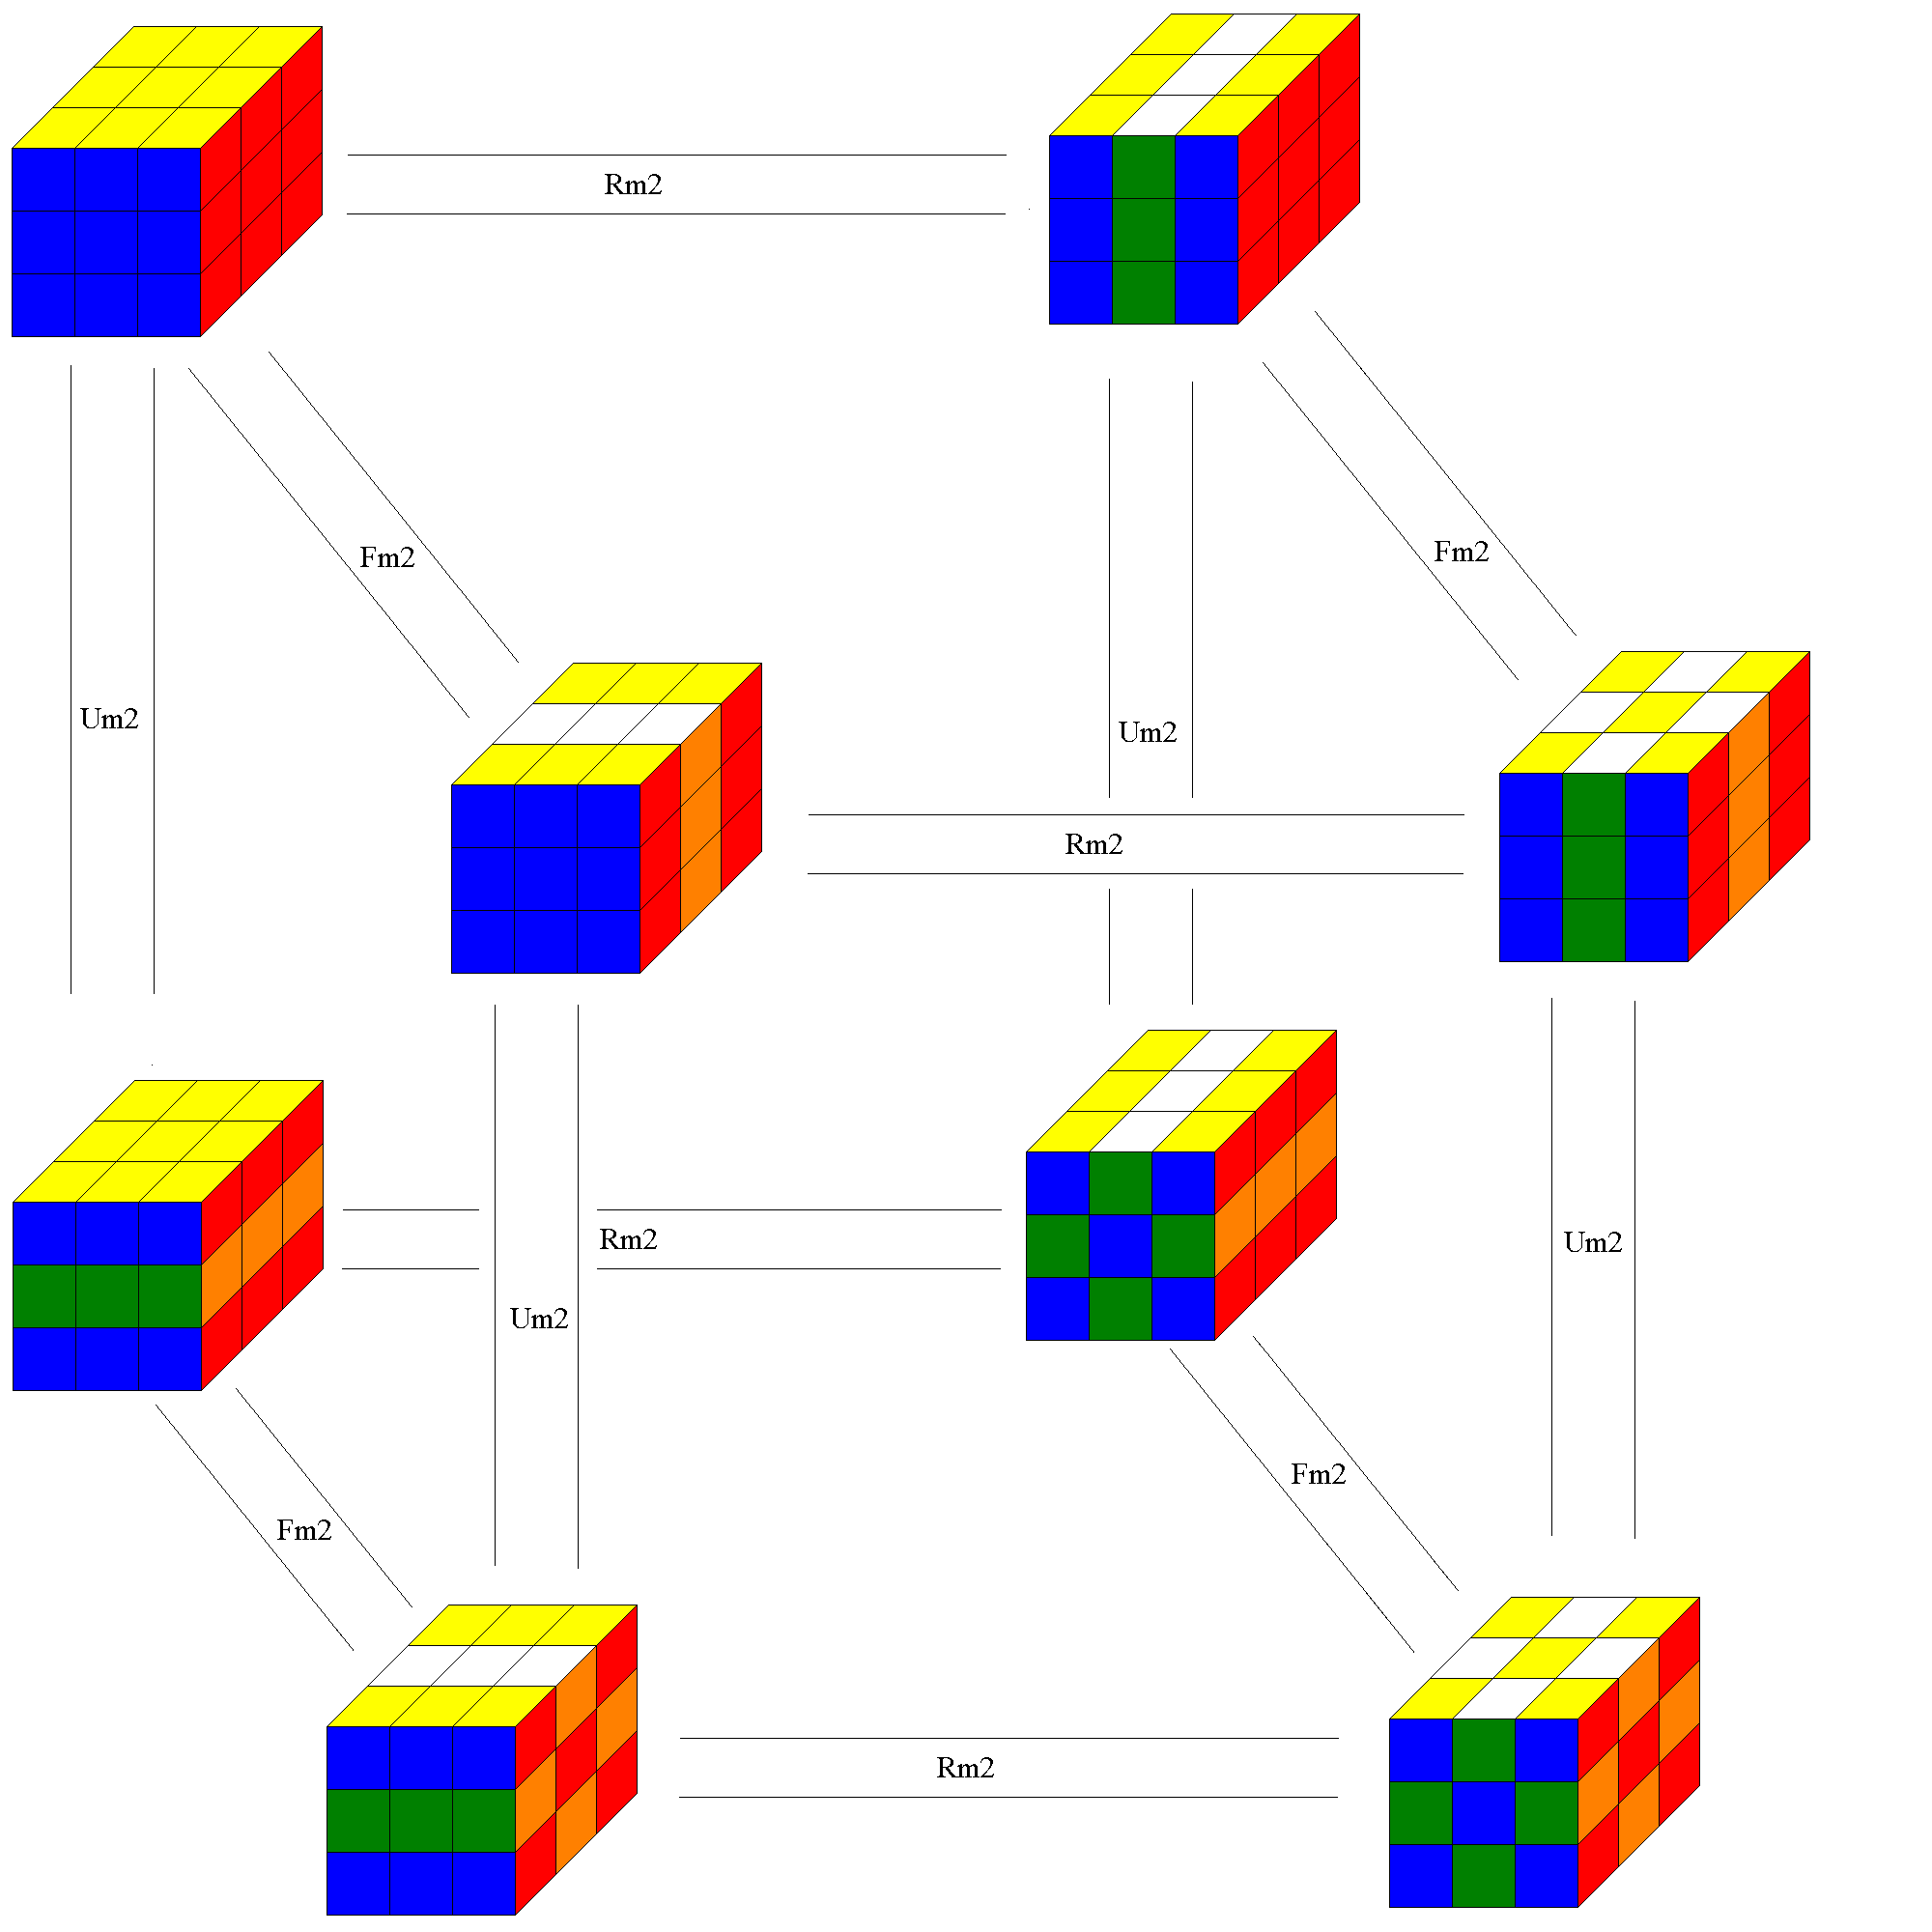
\includegraphics[width = \textwidth]{input/pics/graphMiddleSlice2.PNG}
	\caption{\myCaption{The graph of the middle movement positions.}}
	\label{fig:graphMiddleSlice2}
\end{figure}

Because of this graphs relatively small size the computation of the diameter is a some what simple task. Of course one could calculate the distance from all positions to all other positions. But since the graph is clearly symmetrical one can omit many calculations. It is easy to see that the diameter must go from one corner to an opposite corner e.g. from the solved state to the flip stated. The diameter here is 3. 

In the full cube group it is believed that the analogous position to this flipped position, the superflip position, is the position which has the longest shortest path \cite{speedsolving.wiki}. This has never been proven. This shortest path from the superflip to the solved position is 20.

\myTail{A short general description of graph theory has been presented in this chapter along with a way to calculate the diameter of a graph. For better understanding of the theory, an example on applying the theory on the Rubik's Cube has been shown.}